\documentclass[12pt,a4paper]{article}
\usepackage[utf8]{inputenc}
\usepackage[russian]{babel}
\usepackage[T1]{fontenc}
\usepackage{amsmath}
\usepackage{amsfonts}
\usepackage{amssymb}
\usepackage{graphicx}
\usepackage{wrapfig}
\usepackage[left=2cm,right=2cm,top=2cm,bottom=2cm]{geometry}
\author{Григорий Чирков}
\title{Лабораторная работа №1.3 \\
		 Изучение рассеяния медленных электронов на атомах (эффект Рамзауэра) }

\begin{document}
\maketitle
\section{Теория}
К. Рамзауэр в 1921 г. исследовал зависимость поперечных сечений упругого рассеяния электронов (с энергией до 10 эВ) на атомах аргона. В результате этих исследований было обнаружено явление, получившее название эффекта Рамзауэра. \\

Эффективное сечение реакции (иногда его называют поперечным сече­нием или просто сечением реакции) — это величина, характеризующая вероятность перехода системы двух сталкивающихся частиц в результате их рассеяния (упругого или неупругого) в определенное конечное состояние. Сечение $\sigma$ равно отношению числа $N$ таких переходов в единицу времени к плотности $nv$ потока рассеиваемых частиц, падающих на ми­шень, т. е. к числу частиц, проходящих в единицу времени через единичную пло­щадку, перпендикулярную к их скорости $v$ ($n$ — плотность числа падающих ча­стиц)
\begin{equation}
\sigma = \frac{N}{nv}
\end{equation}
Таким образом, сечение имеет раз­мерность площади. \\

\begin{wrapfigure}{r}{0.4\linewidth} \label{graph} 
\vspace{-5ex}  
 \center{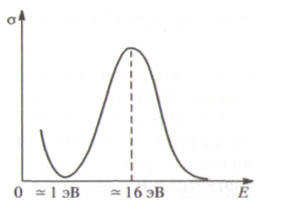
\includegraphics[width=.9\linewidth]{graph.png}}
\caption{Качественная картина ре­зультатов измерения упругого рассеяния электронов в аргоне}
\end{wrapfigure}
Качественно результат экспериментов Рамзауэра при энергии электронов по­рядка десятков электрон-вольт на аргоне показан на рис. \ref{graph}. По мере уменьшения энергии электрона от нескольких десятков электрон-вольт поперечное сечение его упругого рассеяния растет, как это и следует из очень про­cтых рассуждений: чем меньше скорость электрона, тем медленнее он "проскакивает" мимо атома, тем больше время взаимодействия электро­нов с атомом и, тем самым, больше вероятность этого взаимодействия, т. е. сечение реакции. Однако в эксперименте наблюдалось, что при энергиях меньше 16 эВ сечение начинает уменьшаться, а при $E \sim $ 1 эВ практически равно нулю, т. е. аргон становится прозрачным для элек­тронов. При дальнейшем уменьшении энергии электронов сечение рас­сеяния опять начинает возрастать. Объяснение этого эффекта требует  учета волновой природы электронов. \\


\begin{wrapfigure}{l}{0.4\linewidth} \label{scheme} 
 \center{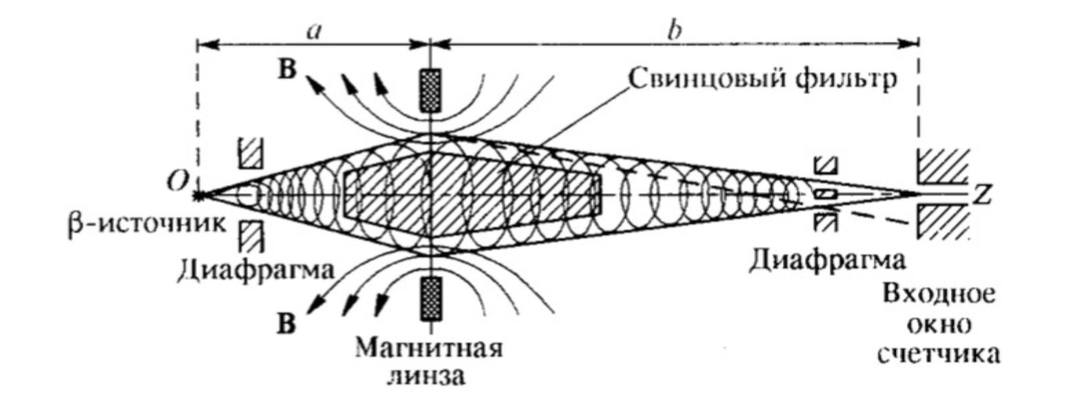
\includegraphics[width=.9\linewidth]{scheme.png}}
\caption{Схема установки для измерения сечения рассеяния электронов в газах}
\end{wrapfigure}
Схема эксперимента Рамзауэра показана на рис. \ref{scheme}.
Пучок электронов, вылетая из накаленного катода К, проходит уско­ряющую разность потенциалов V, приложенную между катодом и элек­тродом Э, и приобретает тем са­мым энергию $E = m v^2 /2 = eV$. При прохождении через газ часть электронов рассеивается на ато­мах, уходит в сторону и собира­ется коллектором КЛ, а прошед­шие без рассеяния электроны попадают на анод А и создают анод­ный ток $I$. Ток $I$ пропорционален числу прошедших электронов, и поэтому непосредственно харак­теризует проницаемость газа для электронного пучка в зависимо­сти от его скорости (ускоряюще­го напряжения). Согласно клас­сическим воззрениям, с ростом напряжения V, как указывалось выше, сечение рассеяния уменьшается, и ток должен монотонно возрастать. \\

С точки зрения квантовой теории картина рассеяния выглядит ина­че. Внутри атома потенциальная энергия налетающего электрона $U$ от­лична от нуля, скорость электрона изменяется, становясь равной $v'$ в соответствии с законом сохранения энергии
\begin{equation}
E = \frac{m v^2}{2} = \frac{m v'^2}{2} + U,
\end{equation}
а значит, изменяется и его длина волны де Бройля. Таким образом, по отношению к электронной волне атом ведет себя как преломляющая среда с относительным показателем преломления
\begin{equation}
n = \frac{\lambda}{\lambda'} = \sqrt{1 - \frac{U}{E}}.
\end{equation}

\begin{wrapfigure}{r}{0.4\linewidth} \label{problem} 
\vspace{7ex}
 \center{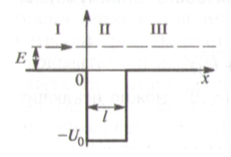
\includegraphics[width=.9\linewidth]{problem.png}}
\caption{Схематическое изображение прямоугольной ямы, над которой пролетает частица с энергией $E$}
\end{wrapfigure}

Для качественного анализа вопроса рассмотрим следующую модель: будем считать, что электрон рассеивается на одномерной потенциальной яме конечной глубины. Фор­му ямы для качественных оценок можно считать пря­моугольной. Модель прямоугольной потенциальной ямы является хо­рошим приближением для атомов тяжелых инертных газов, отличаю­щихся наиболее компактной структурой и резкой внешней границей.

Уравнение Шредингера в данном случае имеет вид:
\begin{equation}
\psi'' + k^2 \psi = 0, 
\end{equation}
где
\begin{equation}
k^2 = 
\begin{cases}
k_1^2 = \frac{2mE}{\hbar^2} & \text{ - в областях I и III}\\
k_2^2 = \frac{2m(E+U_0)}{\hbar^2} & \text{ - в области II}
\end{cases}
\end{equation}

Коэффициент прохождения равен отношению квадратов амплитуд прошедшей и падающей волн и определяется выражением
\begin{equation}
D^{-1} = 1 + \frac{(k_1^2 - k_2^2)^2}{4k_1^2 k_2^2} \sin^2(k_2l) = 1 + \frac{U_0^2}{4E(E+U_0)} \sin^2(k_2l)
\end{equation}

Мы видим, что коэффициент прохождения частицы над ямой имеет, в зависимости от ее энергии, ряд чередующихся максимумов и мини­ мумов. В частности, если $k_2l = \pi$, то $\sin k_2l = 0$ и коэффициент прохож­ дения равен единице, т. е. отраженная волна отсутствует, и электрон беспрепятственно проходит через атом, что является квантовым анало­гом просветления оптики.
Таким образом, коэффициент прохождения электронов максимален при условии 
\begin{equation}
k_2l = \sqrt{\frac{2m(E+U_0)}{\hbar^2}}l = \pi n, n = 1, 2, 3...
\end{equation}

\begin{wrapfigure}{l}{0.4\linewidth} \label{wave} 
 \center{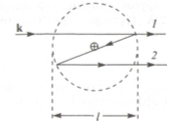
\includegraphics[width=.9\linewidth]{wave.png}}
\caption{Схема интерференции волн де Бройля при рассеянии на атоме}
\end{wrapfigure}
Это условие можно легко получить, рассматривая интерференцию электронныъ волн де Бройля в атоме. Движущемуся электрону соответствует волна де Бройля, длина которой определяется соотношением $\lambda  = h/mv$. Если кинетическая энергия электрона невелика, то $E = mv^2/2$ и $\lambda = h/\sqrt{2mE}$. При движении электрона через атом длина волны де Брой­ля становится меньше и равна $\lambda' = h/\sqrt{2m(E + U_0)}$, где $U_0$ — глуби­на атомного потенциала. При этом, как показано на рис. \ref{wave}, волна де Бройля отражается от границ атомного потенциала, т. е. от поверхно­ стиатома, и происходит интерференция прошедшей через атом волны и волны 2, отраженной от передней и задней границы атома (эти волны когерентны).

Прошедшая волна 1 усилится волной 2, если геометрическая раз­ность хода между ними $\Delta = 2l = \lambda'$, что соответствует условию первого интерференционного максимума, т. е. при условии
\begin{equation} \label{max}
2l = \frac{h}{\sqrt{2m(E_1 + U_0)}}
\end{equation}
Здесь $E_1$ -- энергия электрона, соответствующая этому условию.

С другой стороны, прошедшая волна ослабится, если $\Delta = 2l = (3/2)\lambda'$, т.е. при условии 
\begin{equation} \label{min}
2l = \frac{3}{2} \frac{h}{\sqrt{2m(E_2 + U_0)}}
\end{equation}

Решая совместно эти два уравнения, можно исключить $U_0$ и найти эффективный размер атома $l$
\begin{equation} \label{size}
l = \frac{h \sqrt{5}}{\sqrt{32m(E_2 - E_1)}}
\end{equation}

Понятно, что энергии $E_1$ и $E_2$ соответствует энергиям электронов, прошедших разность потенциалов $V_1$ и $V_2$, т.е. $E_1 = eV_1$ и $E_2 = eV_2$. 

Из формул (\ref{max}) и (\ref{min}) можно также по измеренным величинам $E_1$ и $E_2$ рассчитать эффективную глубину потенциальной ямы атома:
\begin{equation} \label{hole}
U_0 = \frac{4}{5} E_2 - \frac{9}{5} E_1
\end{equation}

\newpage

\section{Установка}

\begin{figure}[ht!]\label{tiratron} 
 \center{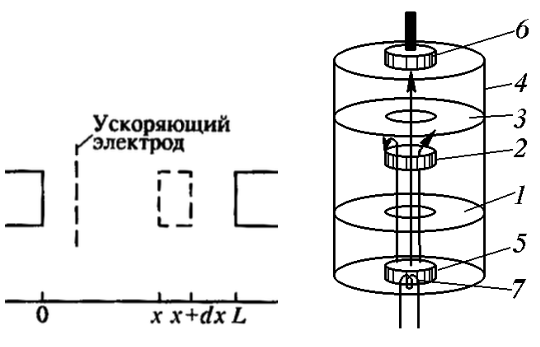
\includegraphics[width=.9\linewidth]{tiratron.png}}
\caption{Схематическое изображение тиратрона (слева) и его конструкция (справа): 1, 2, 3 - сетки; 4 -- внешний металлический цилиндр; 5 -- катод; 6 -- анод; 7 -- накаливаемая спираль}
\end{figure}

Уравнение ВАХ тиратрона:
\begin{equation} \label{VAH}
I_a = I_0 e^{-C\omega(V)}, C = L n_a \Delta_a,
\end{equation}
где $I_0 = e N_0$ -- ток катода, $I_a = e N_a$ -- анодный ток, $\omega(V)$ -- вероятность рассеяния электрона на атоме, $\Delta_a$ -- площадь попереченого сечения атома, $n_a$ -- концентрация атомов газа в лампе, $N_0$ -- поток электронов у катода, $N_a$ -- поток электронов у анода, $L$ -- длина лампы.


\begin{figure}[ht!]\label{omega} 
 \center{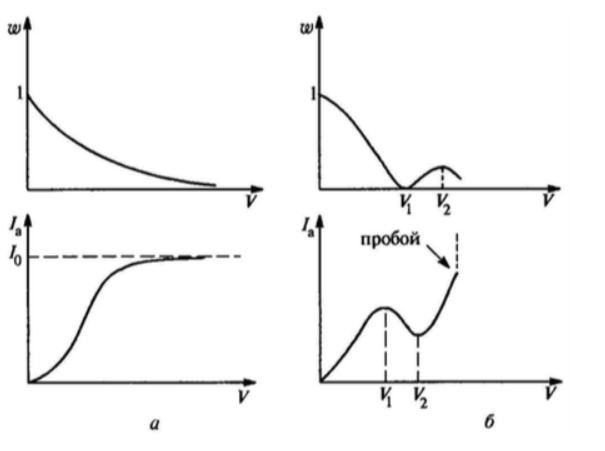
\includegraphics[height=30ex]{omega.png}}
\caption{Качественный вид вероятности рассеяния электрона атомом инертного газа и ВАХ тиратрона при классическом (а) и квантовом (б) рассмотрении}
\end{figure}

Согласно классическим представлениям сечение рассеяния электро­на на атоме должно падать монотонно с ростом V (обратно пропорционально скорости электрона, т. е. обратно пропорционально квадратному корню из его энергии), а значит, ВАХ будет монотонно возрастающей функцией, как это показано на рис. 6а. По квантовым соображениям ве­роятность рассеяния электронов и соответствующая ВАХ должны иметь вид, показанный на рис. 66.

Согласно формуле (\ref{VAH}) по измеренной ВАХ тиратрона можно определить зависимость вероятности рассеяния электрона от его энергии из соотношения
\begin{equation}
\omega(V) = -\frac{1}{C} \log\frac{I_a(V)}{I_0}
\end{equation}

\section{Ход работы}
\begin{enumerate}
\item Снять ВАХ тиратрона в динамическом режиме (на анод подается переменный гармонический сигнал)
\item Снять ВАХ тиратрона в статическом режиме
\item В статическом режиме качественно проследить за изменением ВАХ при поднесенном к тиратрону магните
\end{enumerate}

\section{Обработка результатов}

\begin{enumerate}
\item
$V_{min} \approx 7.5 \pm 1 V$ \\
$V_{max} \approx 2.5 \pm 1 V$ \\
Из формулы (\ref{max}):
$l \approx 2.6 \pm 0.5$ {\AA}

\item
По формуле (\ref{hole}): $U_0 \approx 1.5 \pm 0.4 eV$

\item
Полученное напряжение пробоя $V_\text{проб} \approx 11.3 \pm 0.5 V$ близко к напряжению пробоя ксенона $V_\text{ксенон} = 12.1 V$. Следовательно, газ в тиратроне -- ксенон.

\item Графики статического режима:

\begin{figure}[ht!]\label{omega} 
 \center{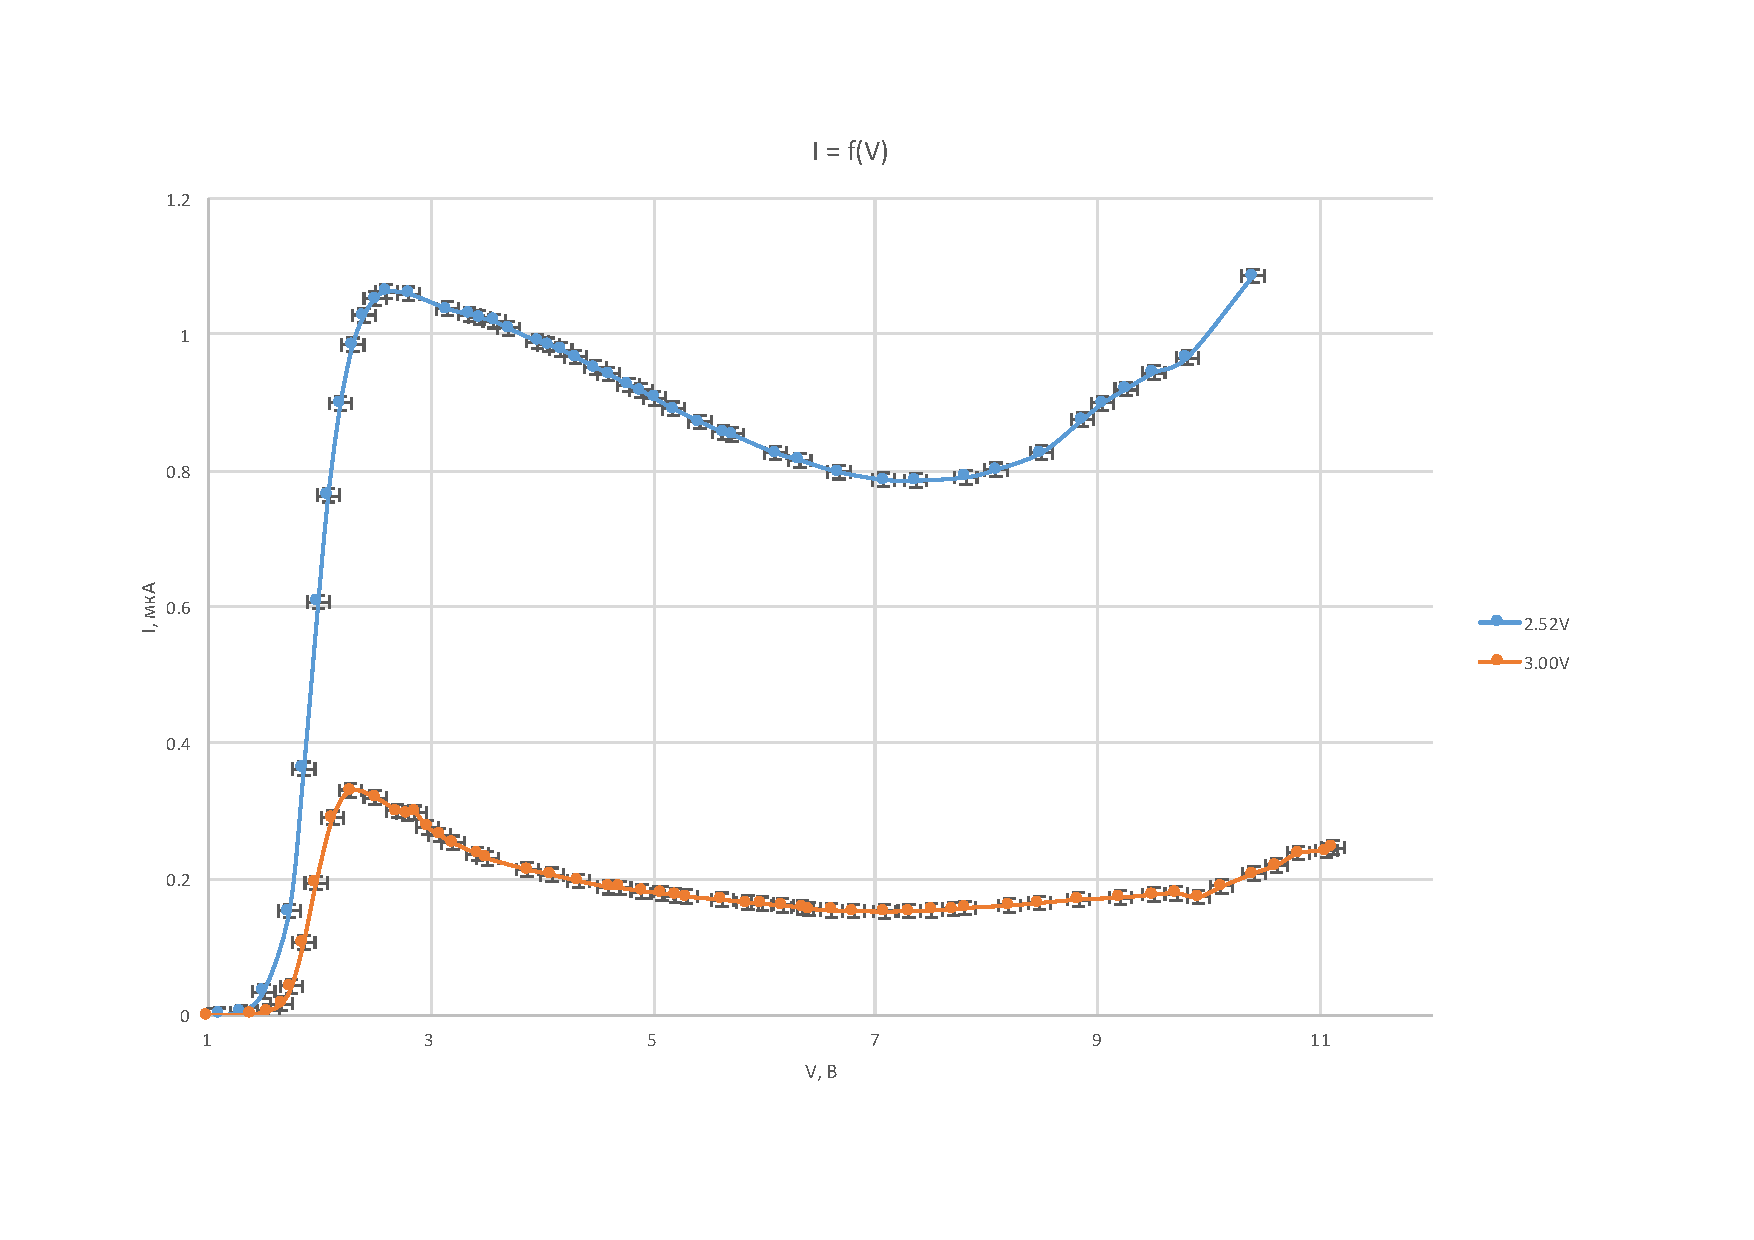
\includegraphics[height=49ex]{I(V).pdf}}
\caption{ВАХ тиратрона в статическом режиме}
\end{figure}
 
 По ним можем определить:
 \begin{itemize}
 \item $V_{min} \approx 7.2 \pm 0.1 V$
 \item $V_{max} \approx 2.4 \pm 0.1 V$
 \item Из формулы (\ref{max}):
$l \approx 2.7 \pm 0.1$ {\AA}
\item 
По формуле (\ref{hole}): $U_0 \approx 1.4 \pm 0.1 eV$
 \end{itemize}

\item Оценим положения следующих максимумов:
\begin{gather*}
k_2l = \sqrt{\frac{2m(E_n+U_0)}{\hbar^2}}l = \pi n, n = 1, 2, 3... \\
\Downarrow \\
\sqrt{\frac{E_n + U_0}{E_1 + U_0}} = n \\
\Downarrow \\
E_n = (E_1 + U_0) n^2 - U_0 \\
E_2 = 17.1 eV \\
E_3 = 41.6 eV
\end{gather*}
\item 
На основе проведенных измерений, построим качественный график зависимости $\omega(V)$:

\begin{figure}[ht!]\label{omega} 
 \center{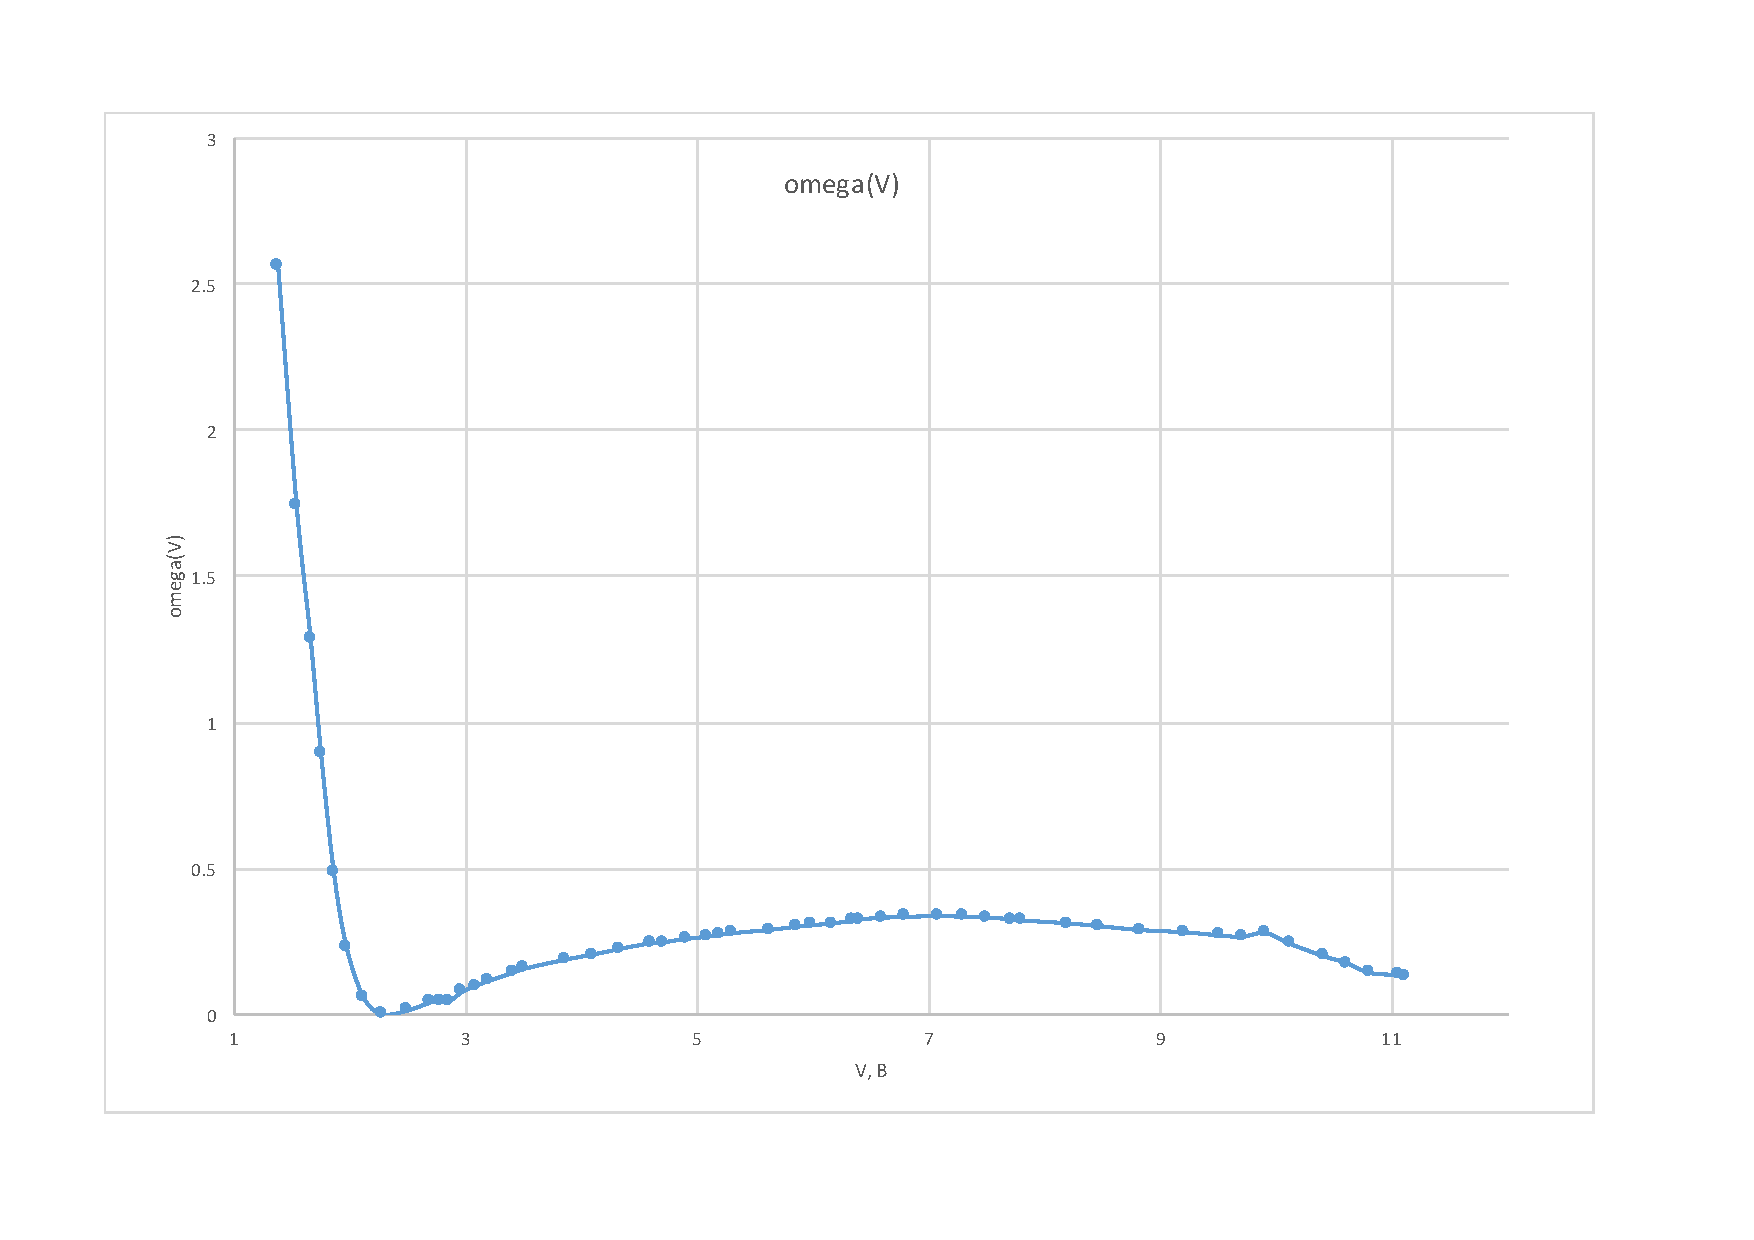
\includegraphics[width=.9\linewidth]{omega.pdf}}
\caption{Зависимость вероятности рассеяния электрона на атоме от его энергии}
\end{figure}
 
\end{enumerate}

\section{Вывод}

В ходе эксперимента было подтверждено, что описание рассеяния электрона на атоме является неточным. Для объяснения эффекта Рамзауэра требуется использовать законы движения квантовой механики. В частности, график зависимости вероятности рассеяния электрона (рис. \ref{omega}) наглядно показывает, как отличается рассеяние электрона в классической механике и квантовой механике.
Полученные значения:
\begin{itemize}
\item $U_0 \approx 1.5 \pm 0.4 eV$ 
\item $l \approx 2.7 \pm 0.1$ {\AA} ( $l_\text{табл} = 1.9$ {\AA})
\end{itemize}
имеют "разумную" величину или совпадают по порядку с табличным значением. 

\end{document}